%Notes by Harsh Mistry 
%Econ 301
%Based on Template From  https://www.cs.cmu.edu/~ggordon/10725-F12/template.tex

\documentclass[twoside]{article}
\setlength{\oddsidemargin}{0.25 in}
\setlength{\evensidemargin}{-0.25 in}
\setlength{\topmargin}{-0.6 in}
\setlength{\textwidth}{6.5 in}
\setlength{\textheight}{8.5 in}
\setlength{\headsep}{0.75 in}
\setlength{\parindent}{0 in}
\setlength{\parskip}{0.1 in}
\usepackage{amsmath,amsfonts,graphicx, color}
\newcounter{lecnum}
\renewcommand{\thepage}{\thelecnum-\arabic{page}}
\renewcommand{\thesection}{\thelecnum.\arabic{section}}
\renewcommand{\theequation}{\thelecnum.\arabic{equation}}
\renewcommand{\thefigure}{\thelecnum.\arabic{figure}}
\renewcommand{\thetable}{\thelecnum.\arabic{table}}
\newcommand{\lecture}[4]{
   \pagestyle{myheadings}
   \thispagestyle{plain}
   \newpage
   \setcounter{lecnum}{#1}
   \setcounter{page}{1}
   
   
%Info Box 
   \begin{center}
   \framebox{
      \vbox{\vspace{2mm}
    \hbox to 6.28in { {\bf Econ 301 - Microeconomic Theory 2
	\hfill Winter 2018} }
       \vspace{4mm}
       \hbox to 6.28in { {\Large \hfill Lecture #1: #2  \hfill} }
       \vspace{2mm}
       \hbox to 6.28in { {\it Lecturer: #3 \hfill Notes By: #4} }
      \vspace{2mm}}
   }
   \end{center}
   
   \markboth{Lecture #1: #2}{Lecture #1: #2}



 
}

\renewcommand{\cite}[1]{[#1]}
\def\beginrefs{\begin{list}%
        {[\arabic{equation}]}{\usecounter{equation}
         \setlength{\leftmargin}{2.0truecm}\setlength{\labelsep}{0.4truecm}%
         \setlength{\labelwidth}{1.6truecm}}}
\def\endrefs{\end{list}}
\def\bibentry#1{\item[\hbox{[#1]}]}

\newcommand{\fig}[3]{
			\vspace{#2}
			\begin{center}
			Figure \thelecnum.#1:~#3
			\end{center}
	}
	
	\graphicspath{ {images/} }

\newtheorem{theorem}{Theorem}[lecnum]
\newtheorem{lemma}[theorem]{Lemma}
\newtheorem{ex}[theorem]{Example}
\newtheorem{proposition}[theorem]{Proposition}
\newtheorem{claim}[theorem]{Claim}
\newtheorem{corollary}[theorem]{Corollary}
\newtheorem{definition}[theorem]{Definition}
\newenvironment{proof}{{\bf Proof:}}{\hfill\rule{2mm}{2mm}}
\newcommand\E{\mathbb{E}}


%Start of Document 
\begin{document}

\lecture{18}{March 19, 2018}{Jean Guillaume Forand}{Harsh Mistry}


\section{Externalities Continued}
\textcolor{blue}{
\textbf{Note :} This lecture builds upon the example in Lecture 17}
\begin{itemize}
\item A competitive equilibrium consists of prices \(p^* = (p_1^*, p_2^*, p_R^*) \) and allocations \(x^{A*} = (x_1^{A*}, x_2^{A*}, x_R^{A*})\)and \(x^{B*} = (x_1^{B*}, x_2^{B*}, x_R^{B*})\) which satisfy 
\begin{enumerate}
\item Given price \(p^*\) and allocation \(X^{A*}\) solves
\[\max_{x_1^{A*}, x_2^{A*}, x_R^{A*} \geq 0} x_1^{A\frac{1}{2}}x_2^{A \frac{1}{2}} \text{ s.t } \hspace{0.2cm} p_1^* x_1^A + p_2^* x_2^A + p_R^* x_R^A \leq 2p_1^* + p_2^* + p_R^* \omega^A_R \]
allocation \(x^{B*}\) solves
\[\max_{x_1^{B*}, x_2^{B*}, x_R^{B*} \geq 0}  x_1^{B\frac{1}{2}}x_2^{B \frac{1}{2}} \text{ s.t } \hspace{0.2cm} p_1^* x_1^B + p_2 x_2^B + p_R^* x_R^B \leq p_1^* + p_2^* + p_R^* \omega_R^B \] 
\item Allocations \(x^{A*}\) and \(x^{B*}\) clear al markets \(x_i^{A*} + x_i^{B*} = \omega_i^A + \omega_i^B \) for all \(i = 1, 3, R\) 
\end{enumerate}
\item Derive a competitive equilibrium by first simplifying the consumers UMP. 
\item In any equilibrium, \(p_R^* > 0\)
\begin{itemize}
\item If \(p_R^* = 0\), consumers B's demand for rights is undefined. 
\item Additionally, \(p_1^* > 0\)
\end{itemize}
\item In any equilibrium, \(p_2^* = 0\)
\begin{itemize}
\item If \(p_2^*  > 0\),then we must have \(x_2^{B*} = 0\) 
\item By (MC2), \(x_2^{A*} = 2\)
\item Due to that fact thet \(x_2^{A*} \leq x_R^{A*}\), we have \(x_R^{A*} \geq 2\)
\item By (MCR), \(x_R^{A*} = 2\) and \(x_R^{B*} = 0\)
\item Due to the fact that \(p_1^*, p_2^* > 0\), \hspace{0.2cm} \(x_R^{A*}\) is never optimal
\end{itemize}
\item In any equilibrium \(x_2^{A*} = x_R^{A*}\)
\begin{itemize}
\item \(x_2^{A*} < x_R^{A*} \) can not be optimal because \(u^A\) is increasing in \(x_2^A\) and \(p_2^* = 0\)
\end{itemize}
\item With these findings we can now rewrite the consumers UMP from the previous example
\[\max_{x_1^J, x_R^J \geq 0}  x_1^{J\frac{1}{2}}x_2^{J \frac{1}{2}} \text{ s.t } \hspace{0.2cm} p_1^* x_1^J  p_2^* x_R^J \leq p_1^* \omega_1^J + p_R^* \omega_R^J\]
\item This gives a standard problem with the demand function : 
\[(x_1^{J*} (p_1^* \omega^J), x_R^{J*}(p_1^* \omega^J)) = 
\left( \frac{p_1^* \omega^J_1 + p_2^* \omega_R^J }{2p_1^*}, \frac{p_1^* \omega^J_1 + p_2^* \omega_R^J }{2p_R^*} \right)\]
\item Normalize \(p_1^* = 1\), (MCR) yields 
\[\begin{aligned}
\frac{2 + p_R^* \omega_R^A}{2p_R^* } + \frac{1 + p_2^* \omega_R^B }{2p_R^*} & = 2 \\
\implies p_R^* &  = \frac{3}{2}
\end{aligned}\]
\item Prices \(p^* = (1, 0 , \frac{3}{2})\) and allocations
\[x^{A*} = \left(1 + \frac{3}{4} \omega^A_R, \hspace{0.2cm} \frac{2}{3} + \frac{1}{2} \omega_R^A, \hspace{0.2cm} \frac{2}{3} + \frac{1}{2} \omega^A_R\right)\]
\[x^{B*} = \left(1 + \frac{3}{4} \omega^B_R, \hspace{0.2cm} \frac{1}{3} + \frac{1}{2} \omega_R^B, \hspace{0.2cm} \frac{1}{3} + \frac{1}{2} \omega^B_R\right)\]
form a competitive equilibrium
\item Given any initial endowments of rights \(x^{A*}\) and \(x^{B*}\) are Pareto-efficient. 
\[\frac{\frac{d}{dx_1^A} u^A(x_1^{A*}, x_R^{A*})}{\frac{d}{dx_R^A} u^A(x_1^{A*}, x_R^{A*})} = \frac{p_1^* }{p_2^*} = \frac{2}{3} = \frac{\frac{d}{dx_1^B} u^B(x_1^{B*}, x_R^{B*})}{\frac{d}{dx_R^B} u^A(x_1^{B*}, x_R^{B*})} \]
\begin{center}
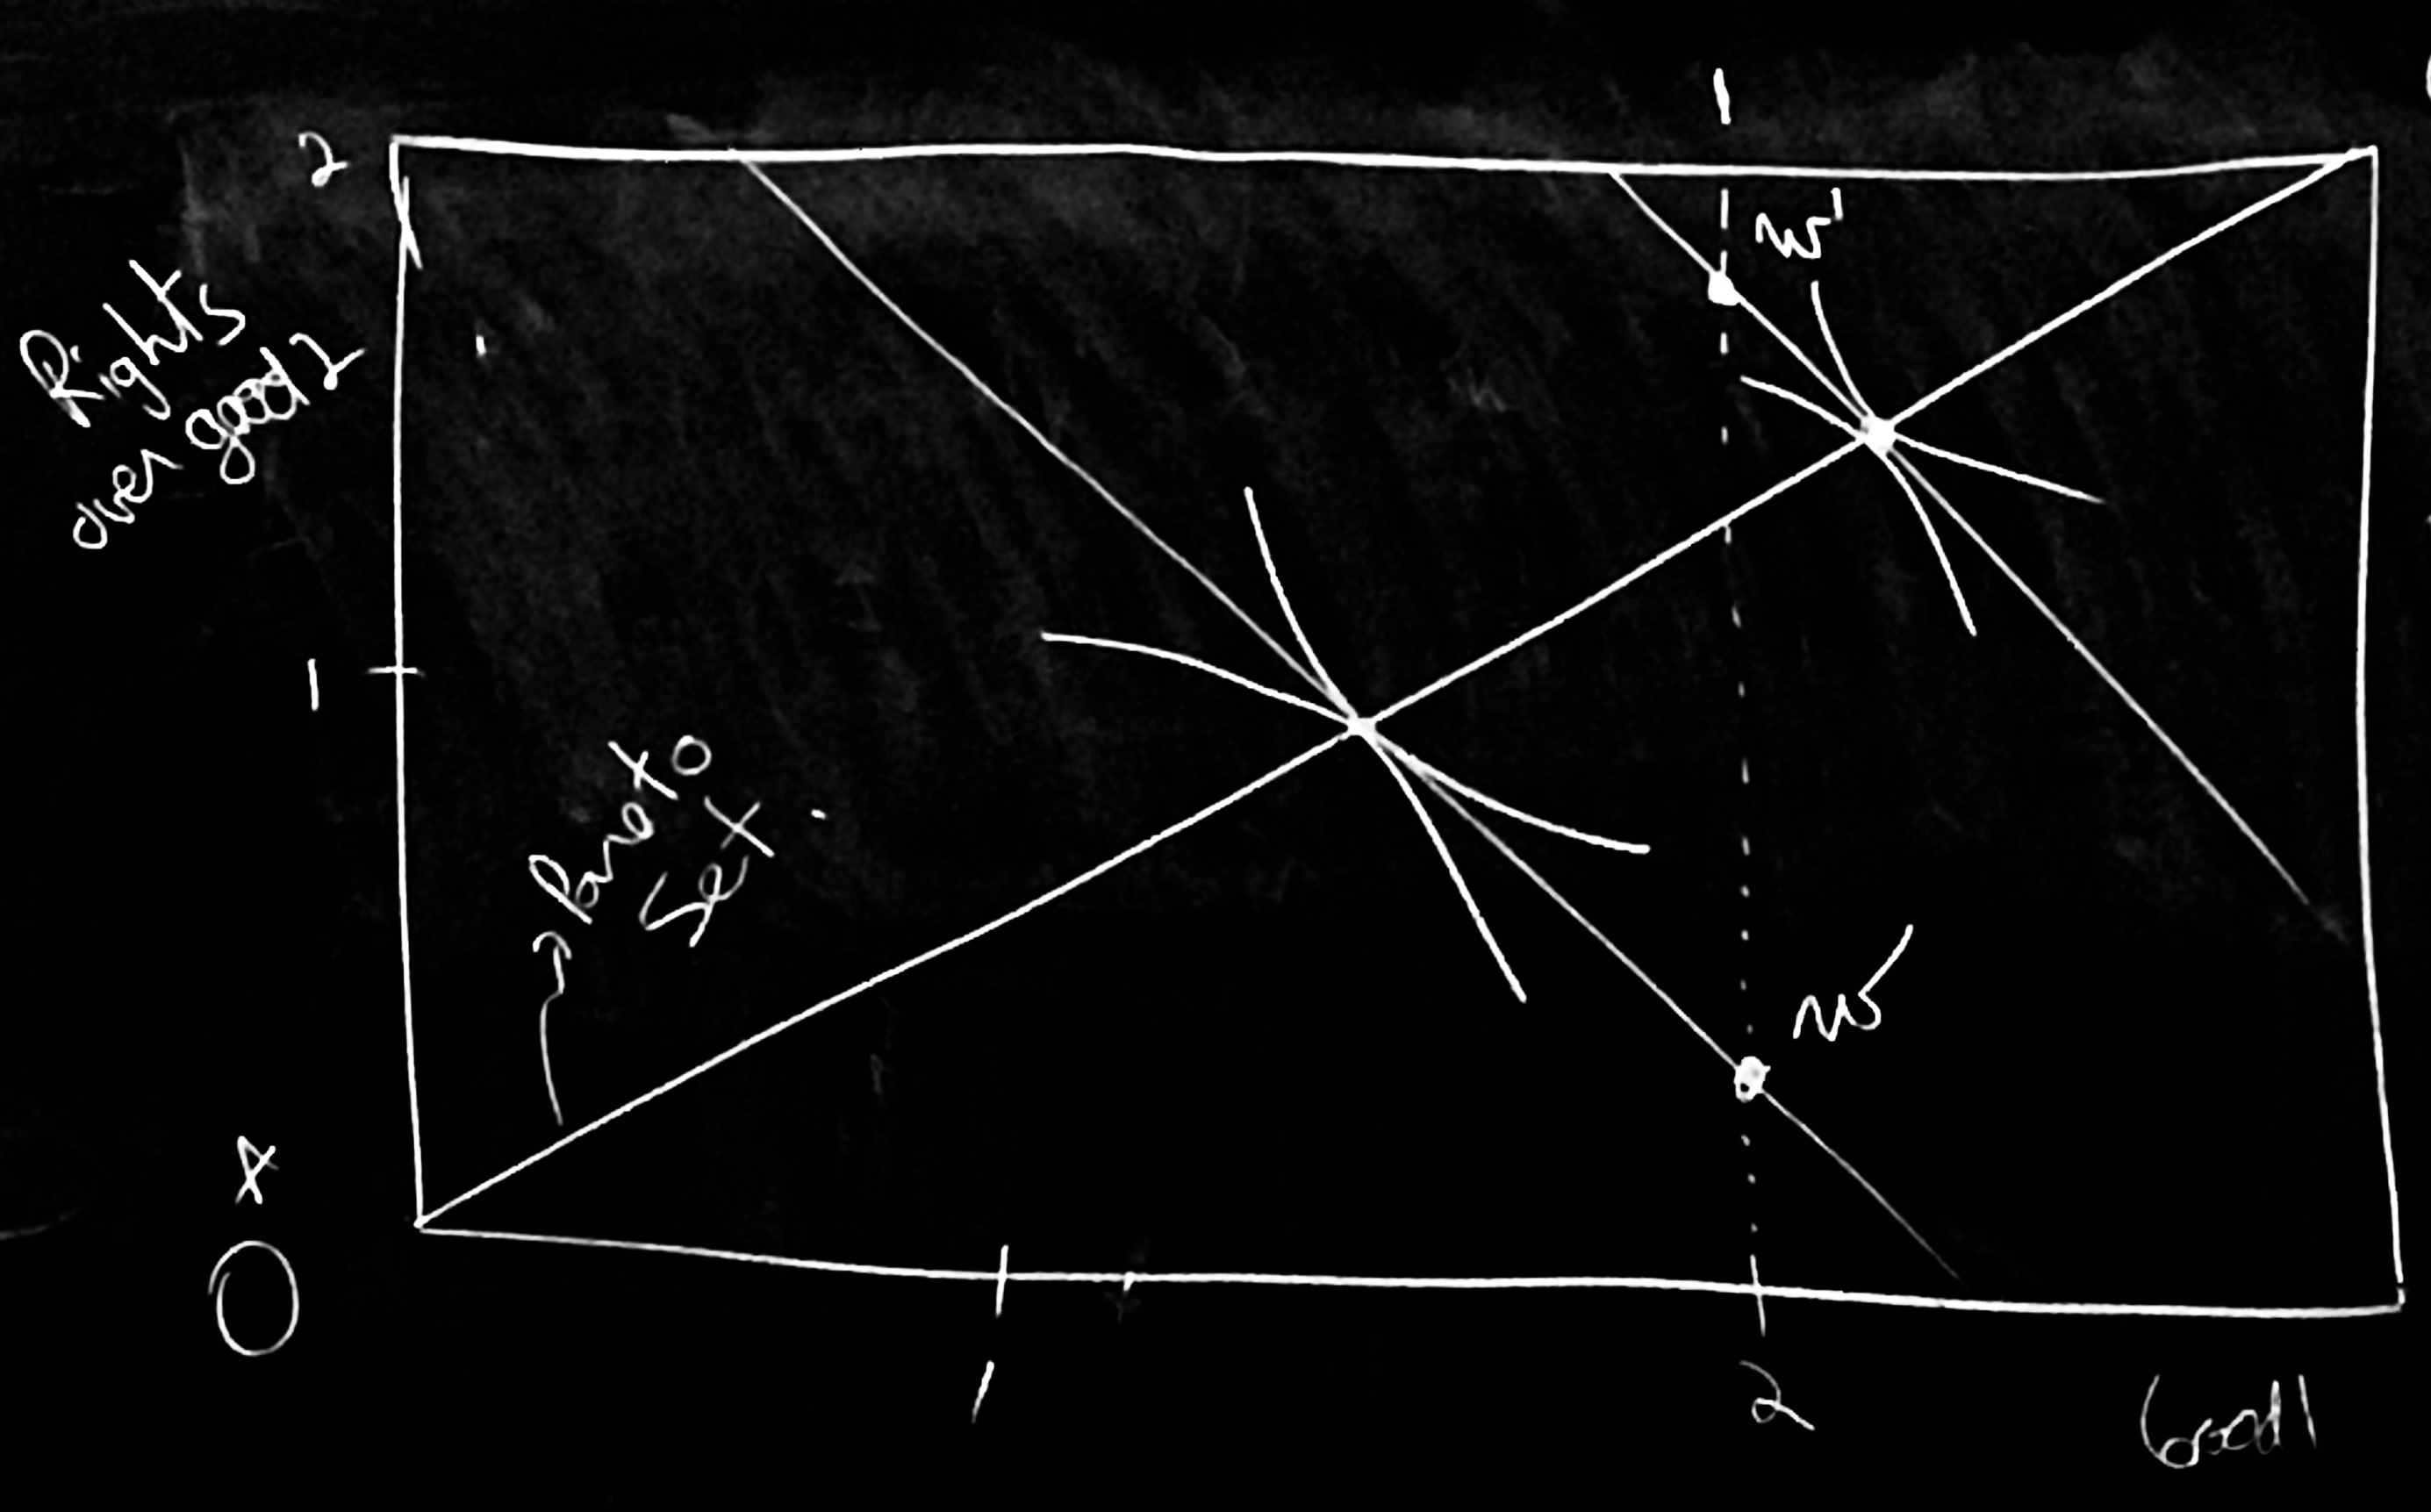
\includegraphics[scale=0.1]{31}
\end{center}
Thus, the Pareto Set is 
\[\left(\frac{x_R^A}{x_1^A}\right) = \left(\frac{2 - x_R^A}{3-x_1^A} \right) \implies x_R^* = \frac{2}{3}x_1^A\]
\item Externalities create missing-market problem, but if property rights are established over externalities, then welfare theorems apply.
\item In practice, completing markets entails the creation of new institutions and distribution of property rights which can be difficult. Additionally, initial allocations have large effects on equilibrium welfare. 
\end{itemize}


\end{document}





